\chapter{Literature Review, Contributions and Scope} 

\label{chap:lit_review} 

\lhead{Chapter 2. \emph{Literature Review, Contributions and Scope}} 

This literature review aims to provide an overview of the field of Graph Signal Processing (GSP) with a particular emphasis on multivariate reconstruction and regression models. First, we will give some historical context for the subject, highlighting the key theoretical advancements and canonical examples, before moving towards the contemporary developments relevant to this thesis. This begins with a basic review of graph filters and kernels, which are foundational building blocks of the methods presented in this thesis. Next, we discuss the topic of graph signal reconstruction, before covering different approaches to regression with graph signals. This is followed by a survey of the emerging field of multiway graph signal processing, and finally, we discuss node classification methods. For each of these topics, we explain how the methods presented in this thesis contribute to the field. 

By presenting a holistic view of the existing literature, this review aims to set a firm foundation upon which we can build the discussion for our ensuing research questions. In addition, this chapter will also hone in on the specific scope of this thesis and define the boundaries of our research. In particular, we aim to identify the areas of interest that remain under-explored or incomplete in the current state of research, as well as demarcate the topics which are not directly relevant to our research focus. 


\section{A historical perspective on GSP}

Though GSP as a field in its own right is generally understood to have been established in the early 2000s, its underlying conceptual framework draws upon the well-established fields of Spectral Graph Theory (SGT), and Digital Signal Processing (DSP), which both date back several decades. SGT is a branch of mathematics that studies the eigenvalues and eigenvectors associated with a graph's adjacency or Laplacian matrix to gain insight into its structural properties \citep{Chung1997}. Early work on SGT can be traced back to the 1950s and '60s \citep{Collatz1957, Hoffman1969}, although many of the concepts had already been studied in parallel within quantum chemistry \citep{Huckel1931}. One of the foundational results in SGT is the multiplicity of the Laplacian's zero eigenvalue gives the number of connected components in the graph \citep{Cvetkovic1980}. Another key result is Cheeger's inequality, which relates the second smallest eigenvalue of the Laplacian (also known as the algebraic connectivity) to the isoperimetric number of the graph (a measure of a graph's bottleneck) \citep{Cheeger1971}. 

Digital Signal Processing (DSP), sometimes considered a branch of electrical engineering, utilises digital computation to analyse, transform, or filter signals, which can be in forms such as sound, images, and sensor data \citep{Rabiner1975}. The core principles of DSP are grounded in linear algebra, calculus, differential equations, and statistics. This theoretical underpinning has led to a plethora of practical applications across varied fields, such as telecommunications, audio processing, image and video processing, astronomy, and seismology, to name a few. Within DSP, the Discrete Fourier Transform (DFT) and its fast algorithmic implementation, the Fast Fourier Transform (FFT), play a central role, with many tasks such as reconstruction, denoising, compression, and filtering requiring analysis and manipulation of the frequency content of signals \citep{Duhamel1990}.

GSP began to take shape as a separate discipline around the start of the 21st century, as the proliferation of data and advancements in computer technology gave rise to more complex, irregular, and high-dimensional data structures. The theoretical framework underpinning GSP emerged from work on Algebraic Signal Processing (ASP), with several papers published by Puschel and Moura from 2003 to 2008 establishing an axiomatic approach to discrete time signal processing \citep{Puschel2003, Puschel2006, Puschel2008}. This mathematical formalism, based on the concept of shift operators, established a unifying framework for several concepts from classical signal processing. For example, under the ASP paradigm, the Discrete Cosine Transform (DCT) and DFT are understood as generated from different discrete shift operators (a chain and cycle respectively) \citep{Isufi2022}. 

Meanwhile, in the data science and machine learning community, concepts from SGT were being applied to nonlinear dimensionality reduction using the Laplacian eigenbasis \citep{Roweis2000, Belkin2003, Donoho2003}. This was followed by work such as \cite{Kondor2002} and \cite{Smola2003}, who studied the topic of graph kernels. This work was subsequently applied in semi-supervised learning, where the goal is to maximise the utility of unlabelled data using its topology in feature space \citep{Belkin2004, Zhou2004, Zhu2003}. We return to the topic of graph kernels in greater detail in \cref{sec:graph_kernels}. 

Around the same time, in the signal processing community, authors were working on both distributed and global algorithms for denoising and regression on sensor networks \cite{Guestrin2004, Wagner2005, Wagner2006}. 

In the early 2010s, two distinct yet complementary approaches to GSP emerged, as discussed in \cite{Leus2023}. The first approach, often credited to \cite{Sandryhaila2013, Sandryhaila2013b}, adopted an algebraic perspective, building upon existing work in Algebraic Signal Processing. This methodology primarily focused on defining the Graph Fourier Transform and related concepts using the foundational operation of graph shifts. Conversely, the second approach, as proposed by  \cite{Hammond2011, Shuman2013}, endorsed the use of the graph Laplacian as the core component for GSP algorithms. This second paradigm, which aligns closely with the concepts presented in \cref{sec:fundamentals}, is also the primary approach utilised in this thesis.


\section{Graph kernels and graph filters}

\label{sec:graph_kernels}

In GSP, two distinct but closely related concepts are graph filters and graph kernels. In the Laplacian-based GSP paradigm, both can be understood as spectral operators which modify the frequency profile of a graph signal, providing a direct generalisation of conventional filters in classical signal processing. (It is worth noting that, in this context, `graph kernel' should not be confused with another concept, bearing the same name, which refers to distance measures between pairs of graphs \citep{Kriege2020}.) Graph filters/kernels play a fundamental role in GSP, and are at the heart of numerous algorithms including reconstruction \citep{Romero2017b}, anomaly detection \citep{Xiao2021}, GNNs \citep{Gama2020} and graph learning \citep{Mateos2019}. 

A graph filter or kernel is characterised by a function $g(\lambda)$, which is applied to the frequency profile of a signal $\y$. This is performed by initially transforming $\y$ into the frequency domain via the GFT, then subsequently applying $g(\cdot)$ to each frequency component independently, and finally transforming back to the node domain via the IGFT. Consequently, it can be represented by a matrix operator $\HH \in \R^{N \times N}$ as follows.

\begin{equation}
    \HH  = \U g(\LAM) \U^\top 
\end{equation}

\begin{table}[t]
    \vspace*{0.5cm}
    \centering
    \setlength{\tabcolsep}{10pt}
    \def\arraystretch{1.8}
    \begin{tabular}{@{}l c@{}}
        \toprule
        \textbf{Filter}   & $g(\lambda; \,\beta)$   \\
        \midrule
        1-hop random walk & $(1 + \beta \lambda)^{-1}$ \\
        Diffusion         & $\exp(-\beta \lambda)$\\
        ReLu              & $\max (1 - \beta \lambda, 0)$\\
        Sigmoid           & $2 \big( 1 + \exp(\beta \lambda)\big)^{-1}$\\
        Gaussian          & $\exp \big(-(\beta \lambda)^2\big)$\\
        Bandlimited       & $1, \,\text{if} \; \beta \lambda \leq 1 \; \text{else} \; 0$ \\
        \bottomrule
    \end{tabular}
    \caption[Example graph filter functions]{Some example low-pass graph filter functions}
    \label{tab:iso_filters}
    \vspace*{0.5cm}
\end{table}


Equivalently, $\HH$ can be understood as originating from the direct application of the function $g(\cdot)$ to the Laplacian, represented as $\HH = g(\LL)$. Here, this operation should be interpreted as an analytic function of a matrix, that is, a series sum of matrix powers \citep{Bhatia1997}. The function $g(\cdot)$ can be set such that it promotes certain properties in the output signal. For example, a low-pass filter (such as those specified in \cref{tab:iso_filters}) is a monotonically decreasing function, attenuating the high-frequency content of a signal. In \cref{tab:iso_filters}, we describe each filter by a positive parameter $\beta$ which controls the filter strength, with higher values resulting in more aggressive attenuation of high-frequency content. The choice of filter will depend on the application of interest and may rely on expert domain knowledge about the spectral profile of the graph signals. 

In the GSP community, the term `filter' is typically preferred when referring to this class of operator \citep{Shuman2013}, although some favour the term `kernel' \citep{Ioannidis2016, Romero2017}. Often, the primary practical distinction is that a kernel is an increasing function, used to construct penalty terms in regularised problems, whereas a filter is a decreasing one, interpreted as providing spectral transformations on graph signals. In \cite{Romero2017b}, the authors advocate for the preferential use of the term kernel, arguing that many GSP methods have an elegant interpretation in terms of Reproducing Kernel Hilbert Spaces (RKHSs). Within the machine learning community, where kernel methods and RKHSs are common, the kernel interpretation is typically favoured \citep{Kondor2002, Smola2003}. Regardless, either convention can be used, and in this thesis, we predominantly describe our methods in terms of filters since they provide a more direct correlation with conventional signal processing techniques, offering an intuitive way to manipulate and reason about the spectral content of graph signals.


\subsection{Probability distributions over graph signals}

Spectral operators can be used to define probability distributions over smooth graph signals. An early example of this approach can be found in \cite{Gadde2015}, where the authors propose a Gaussian Random Field (GRF) model for generating graph signals. In particular, they propose a method for vertex sampling that treats signals as random variables drawn from the following underlying multivariate Gaussian distribution.

\begin{equation}
\y \sim \Norm{\zero}{(\LL + \delta \I)^{-1}}
\end{equation}

This probabilistic interpretation offers a principled way of reasoning about graph signals, making the connection between GSP and specific methods from semi-supervised learning more apparent \citep{Zhu2003}. A more general probabilistic framework for graph signal processing is proposed in \cite{Zhang2015}, where distributions are parametrised by graph filters, offering increased flexibility. Once again, graph signals are interpreted as Gaussian Random Fields, however, the covariance structure is expanded to encompass a greater variety of spectral profiles. In particular, the distribution is given by 

\begin{equation}
    \label{eq:gaussian_filter}
    \y \sim \Norm{\zero}{\gamma^{-1} \HH^2}
\end{equation}


where $\HH$ is a generic graph filter. Since $\HH^2 = \U g^2(\LAM) \U^\top$, this distribution can be interpreted as an independent multivariate Gaussian in the Laplacian eigenbasis, where the covariance of the $i$-th basis vector is given by $g^2(\lambda_i)$. Since, for a low pass filter, $g(\cdot)$ is monotonically decreasing, this naturally results in higher probability density placed on smoothly varying graph signals. 


Further insight into this model can be gained from the following considerations. First, start with an independent multivariate normally distributed random variable, denoted as $\y \sim \Norm{\zero}{\I_N}$. Applying a graph filter yields a new signal, $\HH \y$, which has its high-frequency content attenuated in accordance with the properties of the filter. This filtered signal will also be normally distributed, according to $\HH \y \sim \Norm{\zero}{\HH^2}$. Therefore the process of filtering white Gaussian noise is equivalent to drawing from a distribution with mean zero and covariance $\HH^2$, meaning $\HH^2$ can be interpreted as a covariance matrix for generating smooth, normally distributed graph signals. This flexible approach permits the encoding of various beliefs regarding the frequency profile of graph signals. \Cref{fig:random_smooth_uk} displays an example of a random signal drawn from the distribution of \cref{eq:gaussian_filter} using a bandlimited filter.

% \begin{wrapfigure}{r}{0.4\linewidth}
    \begin{figure}[t]
        \vspace*{0.6cm}
	\centering
		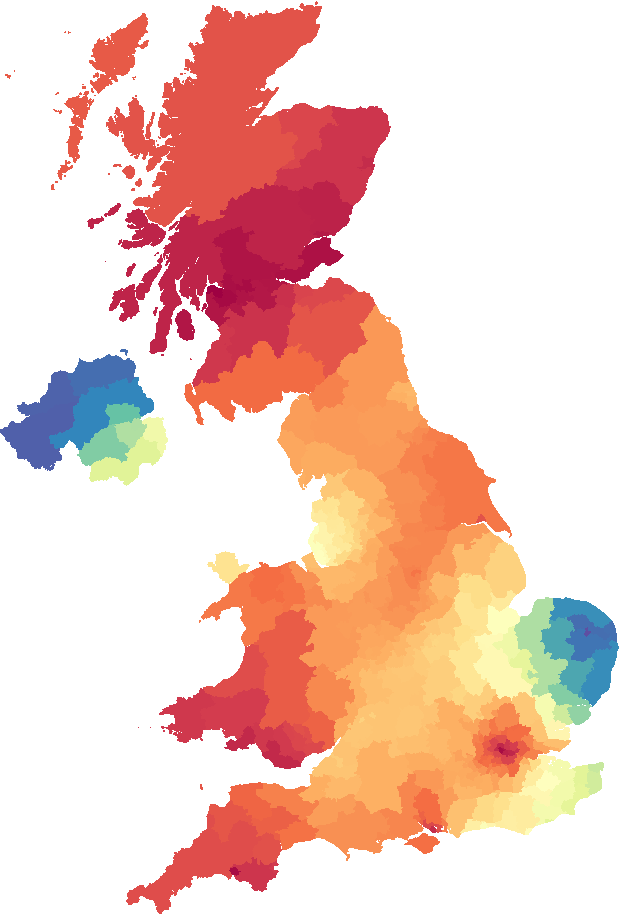
\includegraphics[width=0.4\linewidth]{Figures/uk_smooth.pdf}
	\caption[An example of a random smooth graph signal]{An example of a random smooth signal on the UK district graph, sampled from $\Norm{\zero}{\HH^2}$ using a bandlimited filter. }
	\label{fig:random_smooth_uk}
    \vspace*{0.6cm}
    \end{figure}
% \end{wrapfigure}

This approach is also embraced in \cite{Venkitaraman2020}, where the authors use graph filters to construct a Gaussian process regression model over graphs. In particular, they use a GRF to specify the prior distribution over their weight matrix, resulting in predictions which are smooth with respect to the graph topology. The filter-based GRF model also provides interpretation for the work of \cite{Gadde2015}, which can be seen as a special case of this more general formulation. In particular, their chosen covariance matrix can be written in the form $(\LL + \delta \I)^{-1} = \U g^2(\LAM) \U^\top$, where the filter function is given by $g(\lambda) = 1 / \sqrt{\lambda + \delta}$. Similarly, \citep{Perraudin2017} suggest a flexible class of Laplacian-based covariance matrices, however, their focus is on stationary signals with potentially non-Gaussian distributions. In other work such as \cite{Dong2016}, the authors take a Bayesian approach to the problem of graph learning, using similar graph-spectral priors. 

In general, many types of GSP models utilising some form of quadratic Laplacian-based regularisation can be interpreted in Bayesian terms, although this often goes undiscussed. In this thesis, we follow the example of \cite{Zhang2015} in describing signal distributions with GRFs. However, unlike any of the aforementioned work, we extend this to multidimensional graph signals (two-dimensional matrix signals in \cref{chap:gsr_2d}, and $d$-dimensional tensor signals in \cref{chap:nd_gsp}). This allows us to build a rich class of Bayesian models for tasks such as multivariate reconstruction and regression. 

\subsection{Approximating graph filters with Chebyshev polynomials}

\label{sec:Chebyshev}

So far, we have presented graph filters as spectral operators which are constructed by applying a function to the eigenvalues of the graph Laplacian. However, this formulation is predicated on the notion that it is practical to compute and store the eigendecomposition of $\LL$. Since the time complexity of this operation scales as $O(N^3)$, this can quickly become infeasible for large-scale graphs with a high number of nodes. In addition, applying the matrix $\HH$ to a graph signal has complexity $O(N^2)$, in general requiring information from all nodes to compute the filtered signal value at each node. 

On the other hand, a typical feature of graphs is sparsity, since the degree of each node is often independent of the size of the graph. This means that multiplication of a graph signal $\y$ by the Laplacian can often be achieved with complexity $O(N|\mathcal{E}|) \ll O(N^2)$. Furthermore, in the context of a physically realised graph such as a sensor network, computation of $\LL \y$ can be executed `locally', in the sense that the result at any particular node depends only on the signal value at the direct neighbours of that node. 

One popular and longstanding technique that takes advantage of both these ideas involves approximating a graph filter using Chebyshev polynomials \citep{Shuman2018}. In general, if a graph filter can be approximated as a polynomial of the graph Laplacian, then we can take advantage of the sparsity of $\LL$ to efficiently filter signals without performing eigendecomposition. Consider the following standard polynomial approximation to a graph filter. 

\begin{equation}
    \label{eq:poly_lap}
    g(\lambda) \approx \sum_{k=1}^K c_k \lambda^k \;\; \iff \;\; \HH \approx \sum_{k=1}^K c_k \LL^k
\end{equation}

The Chebyshev polynomial approximation is analogous, but rather than summing powers of $\LL$ directly, we sum order-$K$ polynomials, $\bar{T}_k(\LL)$. 

\begin{equation}
    \label{eq:cheb_lap}
    g(\lambda) \approx \sum_{k=1}^K c_k \bar{T}_k(\lambda) \;\; \iff \;\; \HH \approx \sum_{k=1}^K c_k \bar{T}_k(\LL)
\end{equation}

Standard Chebyshev polynomials form an orthonormal basis with respect to the product

\begin{equation}
    \langle f, g \rangle = \int_{-1}^1 f(x) g(x) \frac{dx}{\sqrt{1 - x^2}}
\end{equation}

and can be used to approximate arbitrary functions within this domain. They also have several well-documented advantages in terms of computational robustness and error over standard polynomial approximations that arise from a Taylor series expansion \citep{Rivlin2020}. While the standard Chebyshev polynomials $\{T_k\}$ are valid on the domain $[-1, 1]$, in the context of graph filters, they must be applicable over the range $[0, \lambda_{\text{max}}]$, leading to the transformed variant $\{\bar{T}_k\}$ appearing in \cref{eq:cheb_lap}. These can be defined recursively as follows. 

\begin{equation}
    \bar{T}_k(\LL) = \left(\frac{4 \LL }{\lambda_{\text{max}}}  - 2\right) \bar{T}_{k-1}(\LL) - \bar{T}_{k-2}(\LL)
\end{equation}

subject to the initial conditions

\begin{equation}
    \bar{T}_0(\LL) = \I_N, \quad \bar{T}_1(\LL) = \frac{2 \LL }{\lambda_{\text{max}}} - \I_N
\end{equation}

Note that this definition ensures only repeated multiplications by $\LL$ when applying $\bar{T}_k(\LL)$ to a graph signal. To approximate an arbitrary filter function $g(\lambda)$, the coefficients $c_k$ are given by 

\begin{equation}
    \label{eq:Cheb_int}
    c_k = \begin{cases}
        \displaystyle   
        \; \frac{1}{\pi} \int_{0}^{\pi} g\left(\frac{\lambda_{\text{max}}}{2} \big(\cos(\theta) + 1\big)\right) \, d\theta  & \quad \text{if} \quad k = 0, \\[0.8cm]
        \displaystyle   
        \; \frac{2}{\pi} \int_{0}^{\pi} \cos(k \theta) \; g\left(\frac{\lambda_{\text{max}}}{2} \big(\cos(\theta) + 1\big)\right) \, d\theta  & \quad \text{otherwise.}
    \end{cases}
\end{equation}

and can be quickly evaluated numerically. 

\begin{figure}[t]
	\centering
		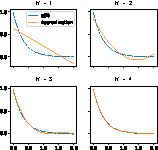
\includegraphics[width=0.55\linewidth]{Figures/cheb.pdf}
	\caption[Successive approximations of a filter function using Chebyshev polynomials.]{Successive approximations of the filter function $g(\lambda) = \exp(-3\lambda)$ using Chebyshev polynomials. }
	\label{fig:Chebyshev}
\end{figure}


Chebyshev polynomials appeared in early papers on GSP, such as \citep{Hammond2011}, in which the authors were concerned with defining wavelet transforms on graphs, also defined in terms of Laplacian-based spectral operators $g(\LL)$. Since then, they have been widely used in distributed applications \citep{Shuman2018}, and have also been extensively employed in Graph Neural Networks \citep{Gama2020}. In \cite{Defferrard2017}, Chebyshev polynomials form the basis of convolutional filters with learned parameters, in direct analogy with traditional Convolutional Neural Networks (CNNs). This approach was further developed in \cite{Kipf2017} by reducing the number of terms in the polynomial to mitigate overfitting.

In \cite{Rimleanscaia2020, Tseng2020}, the authors propose an extension to polynomial filters, which considers a more general class of rational filters, i.e. the ratio between two polynomials. As they describe, in certain circumstances, rational designs can approximate a given frequency response using lower-order polynomials. Notably, when the response is band-limited, rational filters were found to have significantly lower error than standard Chebyshev polynomials, which tend to struggle when approximating the sharp cut-off. In general, rational filtering requires solving a linear system $\y' = P(\LL)^{-1} Q(\LL) \y$, where $P$ and $Q$ are the polynomials occurring in the numerator and denominator, respectively. This incurs an additional computational cost. Furthermore, solving for the coefficients of each polynomial no longer has a closed-form solution and requires addressing a more challenging non-convex, constrained optimisation problem.

As noted, polynomial approximations are primarily useful because multiplications of a graph signal by the Laplacian can be executed efficiently. In all the papers discussed so far, efficiency has been achieved through distributed execution and/or leveraging Laplacian sparsity. However, another way to exploit the Laplacian structure is if it has a representation in terms of a tensor factorisation. In this thesis, we leverage this fact extensively, focusing on how tensor factorisation can further optimise the computation time and resource usage, especially in cases with high-dimensional data or large-scale product graphs.


\section{Graph Signal Reconstruction}

\label{sec:GSR_review}

Graph Signal Reconstruction (GSR), sometimes also known as graph signal interpolation, is a classic problem in GSP \citep{Ortega2018}. The task can be stated as, given a partially observed graph signal, estimate the signal value at the unobserved vertices using only the topology of the graph. Closely related, is the topic of signal sampling, which seeks to find an informative set of vertices to measure a graph signal, in order to perform an accurate reconstruction \citep{Tanaka2020}. GSR is often posed as an optimisation problem where one seeks to identify a smooth underlying graph signal, $\f$, that simultaneously minimises the square error across the observed nodes, as well as a penalty term $P$, that enforces some kind of signal smoothness or bandlimited assumption. 

\begin{equation}
    C(\f) = \sum_{i \in \text{observed}} (\y_i - \f_i)^2 + P(\f)
\end{equation}

Early work on GSR, such as \cite{Narang2013, Wang2015b, Anis2016}, mainly focused on the reconstruction of bandlimited graph signals. Here, the goal is to find the optimal reconstruction of a signal using only the first $K$ eigenvectors of the graph Laplacian, with a frequency less than $\omega$ (the so-called Paley-Wiener space). In \cite{Narang2013}, for example, this is achieved using an Iteratively Reweighted Least Squares (IRLS) algorithm, with a Chebyshev polynomial approximation to the bandlimited filter. While most work assumes that the cut-off frequency is known, some authors have proposed simultaneously learning it \citep{Varma2015, Marques2016}. In other work, such as \citep{Belkin2004b, Narang2013c, Chen2015}, a simpler Laplacian-based regularisation term is used to penalise the total square variation.

In \citep{Romero2017b}, the authors propose using a flexible parametrisation of the reconstructed signal profile based on graph kernels. This can be understood as a generalisation of previous works where, rather than specifying a particular form of the penalty term, arbitrary kernel functions of the graph Laplacian are utilised to draw functions from an RKHS.

Several methods have also been proposed for the reconstruction of time-varying graph signals, in so termed Time-Vertex (T-V) problems. In \cite{Qiu2017}, the penalty term in the optimisation objective promotes both smoothness across the graph using a Laplacian penalty, and consistency across time, by introducing a temporal difference operator $\D$. Despite being presented in a slightly different way, this also amounts to a Laplacian penalty, since $\D\D^\top$, which appears in the regularisation term, is precisely the Laplacian of a path graph. The problem is then solved for both the noiseless and noisy cases using a gradient projection algorithm with a backtracking line search. A similar method is adopted in \cite{Giraldo2022}, but with a regularised version of the Laplacian for improved computational robustness. In \cite{Ioannidis2016}, this approach is modified to incorporate a more dynamic penalty that can adjust the strength of regularisation across the graph and across time independently, using so-termed ``space-time kernels''. Furthermore, in this paper, as well as \cite{Romero2017, Ioannidis2018}, the authors propose an online algorithm that can accommodate dynamic graphs (i.e. graphs for which the edge weights can change over time), although this is only possible for a special class of kernel which have a tri-diagonal inverse. 

Recently, some methods have also been proposed for distributed reconstruction of time-varying graph signals. In \cite{Chi2022}, as well as \citep{Zhou2022b}, the authors propose distributed algorithms that draw upon the work of \cite{Qiu2017} using the temporal difference operator. In these two papers, which have similar goals but were developed separately, the authors use a modified Newton method to solve the optimisation problem, by making use of an approximation to the Hessian. 

In general, there is certainly scope for extensions to the literature on graph signal reconstruction. For example, there are open questions on the best way to address GSR for directed graphs, multilayer graphs and signals where the graph must be learned simultaneously. In particular, we would like to highlight that multidimensional graph signals have only been addressed in the context of time-varying signals. To the best of our knowledge, reconstruction on general Cartesian product and multiway graphs has not been addressed. 



\section{Graph Signal Regression}

Another key topic that runs through this thesis is graph signal regression. One of the earliest papers to reference regression in the context of GSP is \cite{Guestrin2004}. Here, the authors propose a distributed algorithm for computing a function that approximates a time-varying graph signal, with applications aimed specifically at sensor networks. This paper, which predates much of the work on Laplacian-based GSP, is primarily focused on efficient algorithms for communication between sensors, and in modern parlance is more akin to graph signal compression, as the authors seek a low-dimensional representation of the original signal. It can also be considered a particular class of distributed spatial regression, as they consider the $x$-$y$ coordinates of each sensor, rather than modelling the network in terms of nodes and edges. 

In this thesis, the definition of graph signal regression we use differs somewhat from this formulation. For our purposes, we consider graph signal regression to be the task of estimating a graph signal as a function of additional explanatory variables. In particular, we highlight two different scenarios which we term exogenous (global) and endogenous (local) regression. For the exogenous case, we examine work on Kernel Graph Regression (KGR) \citep{Venkitaraman2019} and related variants such as Gaussian Process on Graphs (GPoG) \cite{Venkitaraman2020}. For the endogenous case, we examine work on Regression with Network Cohesion (RNC) \citep{Li2019}. 


\subsection{Exogenous case: Kernel Graph Regression and Gaussian Processes on Graphs}

The task of graph regression with endogenous explanatory variables can be stated as follows. Consider a series of $T$ real-valued graph signals, each measured on a graph comprising $N$ nodes, $\{\y_t \in \R^N\}_{t=1}^T$. Each of these signals has a corresponding associated length-$M$ vector of explanatory variables $\{\x_t\}_{t=1}^T$. The goal is to learn a function that maps the explanatory variables to the graph signals, such that if a new explanatory vector $\x'$ is supplied, we should be able to estimate the corresponding graph signal $\y'$. By penalising predictions that are not smooth with respect to the topology of the graph, the intention is to produce an estimator that outperforms non-graph-aware alternatives. Note that, while we use the index $t$ to denote each sample, the set $\{\x_t, \y_t\}$ can simply be regarded as training pairs and need not represent time-series data (although they often may). 


In this context, the variables are `exogenous' or global in the sense that they are not associated with any node in particular, and the signal at each node in the graph can learn a unique functional response. For example, consider a time-varying graph signal consisting of net profits for a network of businesses connected based on industry or supply chain. In this case, the explanatory variables could be factors in the broader economy such as GDP growth, inflation or unemployment which may affect each company differently. 

In \cite{Venkitaraman2019}, the authors propose Kernel Graph Regression (KGR) for this purpose. Here, each node in the observed graph signal $\y_t$ is modelled as a unique linear combination of a basis function representation of the explanatory variables $\boldsymbol{\phi}(\x_t) \in \R^P$, such that $\y_t = \W^\top \boldsymbol{\phi}(\x_t)$, where $\W \in \R^{P \times N}$ is a matrix of coefficients. To find the optimal value of $\W$, they propose the following cost function. 

\begin{equation}
    C(\W) = \sum_{t=1}^T ||\y_t - \W^\top \boldsymbol{\phi}(\x_t) ||_2^2 + \alpha \tr{\W^\top \W} + \beta \sum_{t=1}^T \text{TV}_2\big(\W^\top \boldsymbol{\phi}(\x_t)\big)
\end{equation}

The first term in this objective seeks to minimise the square prediction error, the second provides regularisation for the coefficient matrix, and the third utilises the total square variation, of \cref{eq:TSV2}, to promote signal smoothness. Next, the authors leverage the so-called `kernel trick' to transform this into a non-parametric regression problem. This is achieved by introducing a $T \times T$ kernel matrix $\K$, where $\K_{ij} = \kappa(\x_i, \x_j)$ \citep{Rasmussen2005}, which results in the following in-sample prediction. 

\begin{equation}
    \mat{\big(\I_N \otimes \K\big)\big(\I_N \otimes (\K + \alpha \I_T) + \beta \LL \otimes \K \big)^{-1} \vecc{\Y}}
\end{equation}

where $\Y \in \R^{T \times N}$ is the matrix formed by stacking each observed signals $\{\y_t\}$, $\vecc{\cdot}$ represents column-major vectorisation mapping $\R^{T \times N} \mapsto \R^{TN}$, and $\mat{\cdot}$ is the reverse operation $\R^{TN}\mapsto  \R^{T \times N}$. The result is the prediction made over the training samples $\{\x_t\}_{t=1}^T$. This can also be adjusted to make a prediction for an unseen explanatory variable $\x'$. Some recent extensions have been proposed to KGR such as \cite{Elias2022}, where the authors use an algorithm based on random Fourier features to improve computational robustness. 

In \cite{Venkitaraman2020}, the same authors propose a new model which takes a Bayesian perspective to define Gaussian Processes over Graphs (GPG). Here, a modified approach is used, where a graph-spectral prior is placed over the coefficient matrix to induce smoothness in the output signal. This results in not only a point estimate for the signal but a multivariate Gaussian probability distribution with a mean and covariance. In particular, the authors define an online algorithm where the distribution over a signal at time $T+1$, given $\x_{T+1}$ is given by 

\begin{equation}
     \Norm{\muu = \D^\top \C_T^{-1}\,\vecc{\Y}}{\; \SIG = \F - \D^\top \C_T^{-1} \D}
\end{equation}

with

\begin{align}
    \C_T &= \HH^2 \otimes \K + \beta^{-1} \I_N \otimes \I_T \\[0.1cm]
    \D &= \HH^2 \otimes \big[\kappa(\x_1, \x_{T+1}), \, \kappa(\x_2, \x_{T+1}), \, ... \, ,\, \kappa(\x_N, \x_{T+1})\big]^\top \\[0.1cm]
    \F &= \kappa(\x_{T+1}, \x_{T+1}) \HH^2 + \beta^{-1} \I_N
\end{align}

Several papers have also proposed extensions to this model. For example, in \cite{Miao2022}, the authors present a modified algorithm that simultaneously learns the underlying graph structure. In \cite{Zhi2023}, the authors propose parametrising the filter function as a finite polynomial of the graph Laplacian, and simultaneously learn the polynomial coefficients, extending their earlier work in \cite{Pu2021}. 

In \cref{chap:kgr_rnc_2d}, we present a hybrid model that incorporates aspects of graph signal reconstruction, as well as Gaussian processes over graphs. In particular, we are interested in reconstructing time-varying partially observed graph signals when additional exogenous explanatory variables exist. Notably, all the models discussed in this subsection assume that readings across all vertices are available as inputs into the model. However, in many real-world applications, node-level data may be corrupted by equipment failure or difficult/expensive to reliably collect. Whilst one option may be to simply remove problematic nodes from the problem entirely, this can waste valuable data that may help in the estimation problem. In \cref{chap:nd_gsp}, we take this further by developing a model that is capable of reconstructing $d$-dimensional multiway graph signals with exogenous variables. To the best of our knowledge, none of these issues have been addressed in the available literature. 


\subsection{Endogenous case: Regression with Network Cohesion}

The second graph regression setting we wish to highlight is the case when endogenous variables exist to aid with the estimation process. Consider a single graph signal $\y \in \R^N$, with elements existing on the nodes of a known graph. In this scenario, each node, $n$, has an associated vector of explanatory variables $\x_n \in \R^M$. The goal is to build a predictive model which utilises these local explanatory variables, whilst also incorporating the underlying structure of the network. 

In \cite{Li2019}, the authors propose Regression with Network Cohesion (RNC). Here, they propose modelling each element of the observed graph signal $\y_n$ as a linear combination of an intercept term and the explanatory variables at node $n$. This is summarised by the following statistical model. 

\begin{equation}
    \y = \cc + \X \w + \boldsymbol{\epsilon}
\end{equation}

$\X \in \R^{N \times M}$ is the matrix formed by stacking each vector of explanatory variables, $\w \in \R^M$ is a coefficient vector, and $\cc \in \R^N$ is a flexible intercept term of individual node effects. The model error $\boldsymbol{\epsilon} \in \R^N$ is assumed to have a zero mean and a variance of $\sigma^2 \I_N$. The model seeks to learn an optimal value for $\cc$ and $\w$ by minimising the following objective function. 

\begin{equation}
    \label{eq:RNC_objective}
    C(\cc, \w) = ||\y - \X \w - \cc ||^2_2 + \lambda \text{TV}_2(\cc)
\end{equation}

The addition of the total square variation term, which the authors name the cohesion penalty, is intended to promote smoothness over the flexible intercept with respect to the topology of the graph. The justification for this is that closely connected nodes are likely to have similar baseline effects, meaning the model simultaneously learns a shared coefficient vector $\w$, and a unique but smooth intercept. The optimal values can be computed by introducing a combined parameter vector $\thetaa = \begin{bmatrix} \cc \\ \w  \end{bmatrix}$, with an estimator given by 

\begin{equation}
    \label{eq:theta_RNC_OG}
    \hat{\thetaa} = \begin{bmatrix}
        \I_N + \lambda \LL & \X \\ \X^\top & \X^\top \X
    \end{bmatrix}^{-1} \begin{bmatrix}
        \I_N & \X
    \end{bmatrix} \y
\end{equation}

To make a prediction on the test set, where the new explanatory variables $\X' \in \R^{N' \times M}$ are available, the authors use the following. 

\begin{equation}
    \hat{\y}' = \hat{\cc}' + \X' \hat{\w}
\end{equation}

where $\hat{\w}$ is the optimal value found by minimising \cref{eq:RNC_objective}, and $\hat{\cc}'$ is found by minimising the following objective. 

\begin{equation}
    \hat{\cc}' = \underset{\cc'}{\text{argmin}} \quad \begin{bmatrix}
        \hat{\cc} \\ \cc' 
    \end{bmatrix}^\top \begin{bmatrix}
        \LL_{11} & \LL_{12} \\ \LL_{12}^\top & \LL_{22}
    \end{bmatrix} \begin{bmatrix}
        \hat{\cc} \\ \cc' 
    \end{bmatrix} = - \LL_{22}^{-1} \LL_{12}^\top \hat{\cc}
\end{equation}

where the new Laplacian characterising the full graph containing all train and test nodes has been broken into blocks as shown. Note that as long as the two parts of the graph are mutually connected, the inverse of $\LL_{22}$ will exist. As noted by the authors, there may be some issues surrounding computational robustness within this model. In particular, the system matrix found in \cref{eq:theta_RNC_OG} may in general be singular. To overcome this the authors propose adding a small term $\gamma \I_N$ to the graph Laplacian, which fixes this issue. 

One limitation of the RNC model is that the total square variation penalty, while simple and easy to interpret, lacks the flexibility to specify more generic expectations about the spectral profile of the observed graph signal. Furthermore, the authors only consider a single measurement across the graph, without extending this to time-varying or general multivariate graph signals. 


\section{Multiway Graph Signal Processing}

Multiway Graph Signal Processing (MWGSP) is an emerging subfield that extends Graph Signal Processing to analyse data represented by multidimensional arrays and tensors \citep{Stanley2020}. In most standard GSP applications, a signal is represented by a vector $\y \in \R^N$, which is interpreted as existing on the nodes of a single graph. MWGSP generalises this by considering tensor-valued signals $\Yt \in \R^{N_1 \times N_2 \times ... \times N_d}$, where each axis is described by an independent graph, which are combined together via a $d$-dimensional product. Many multidimensional models and algorithms from GSP and classical signal processing, such as the 2D DFT and Time-Vertex (T-V) signals can be reinterpreted under the MWGSP framework, bringing additional insight and new applications. As a relatively new paradigm, there is yet to be a large pool of research on MWGSP. Whilst many authors have noted its potential applications \citep{Marques2020b,Li2023}, many models from GSP are yet to be discussed in the context of GSP. This leaves many opportunities for the development of theory in this area. 

\begin{figure}[t]
    \centering
    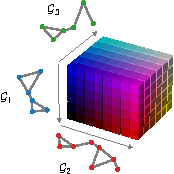
\includegraphics[width=0.45\linewidth]{Figures/colored_tensor.pdf}
    \caption[Graphical depiction of an order-3 tensor]{Graphical depiction of an order-3 tensor signal with graphs underlying each axis.} 
    \label{fig:coloured_tensor}
\end{figure}   

It should be noted that MWGSP is related by distinct from multi-layer GSP \citep{Zhang2023b}. This is also an emerging framework that uses the language of tensors to describe higher-order graph structures. However, in multi-layer GSP, the focus is on multiple layers of heterogeneous graphs, each with possibly different structures and physical meanings, that connect to each other in more general ways. For example, one layer could represent a network of cloud computing servers, and another could represent a power grid. Each layer may have different nodes with \textit{intralayer} edges, and the two layers may be connected via \textit{interlayer} edges. This is certainly a promising and interesting framework, but not the focus of this thesis. 

% \cite{Smilde2004}

% \cite{Kroonenberg2008}

% \cite{Ji2019}

% \cite{Cammoun2009}

% \cite{Li2012}

% \citep{Sandryhaila2014}



\section{Node classification}

The majority of models and algorithms discussed in this review thus far have primarily dealt with real-valued graph signals $\y \in \R^N$. However, it is natural to generalise this to other forms of data, for example, binary signals $\y \in \{0, 1\}^N$ representing two distinct classes, or signals on the interval $\y \in [0, 1]^N$ which could represent probabilities. Moreover, this can easily be extended to categorical data, where each node belongs to one of $C$ classes, with a corresponding simplex representing their respective probabilities. Signals with these characteristics can be employed to design node classification algorithms. 

The GFT operator is typically defined to act on real-valued graph signals, which has conventionally limited GSP models to this type of data. However, some studies have considered node classification tasks. For instance, in \cite{Sandryhaila2013a}, the authors utilise graph signals of the form $\s \in \{-1, 0, +1\}^N$ to represent a binary classification task, with zero signifying an unknown label. Their proposed prediction for the true signal is the solution to the optimisation problem outlined as follows:

\begin{equation}
    \hat{\y} = \argmin{\y \in \R^N} \text{TV}_\text{G}(\y), \quad \text{s.t.} \quad ||\C \y - \C \s ||^2_2 < \epsilon
\end{equation}

Here, $\C$ represents a diagonal matrix with $\C_{nn} = |\s_n|$, and $\text{TV}_\text{G}(\y)$ is a graph shift total variation measure, imposing a smoothness assumption, given by

\begin{equation}
    \text{TV}_\text{G}(\y) = \frac{1}{||\y||^2_2} \left| \left| \y - \frac{1}{\lambda_{\text{max}}} \A \y \right| \right|^2_2
\end{equation}

for a graph adjacency matrix $\A$ with maximum eigenvalue $\lambda_{\text{max}}$. The authors also compare this with a method utilising $\text{TV}_2$ Laplacian-based regularisation, with the results favouring the former approach. One potential issue with this model is that the optimisation searches in the space of real-valued signals, which are subsequently interpreted as estimates for class probabilities. Although the $\epsilon$-condition ensures that the predictions do not deviate excessively from the observed classes, confined to the set $\{-1, 0, +1\}$, there is, in theory, nothing preventing the estimates from extending beyond this range, which may make results difficult to interpret. Furthermore, their total variation measure lacks the flexibility to encode more precise assumptions about the spectral profile of the signal and is applied directly to a class probability vector, which is typically designed for real-valued signals only. This makes some aspects of their model difficult to interpret from a theoretical perspective. 

More recently, \cite{Tran2020} propose a method for binary node classification based on the so-called logistic network lasso. They consider the situation where each node also has an associated vector of explanatory variables $\x_n \in \R^M$, and propose that the class probabilities can be estimated using a logistic function as follows. 

\begin{equation}
    p(\y_n = 1) = \frac{1}{1 + \exp \left(-\w_n^\top \x_n \right)}
\end{equation}

This is similar in spirit to traditional logistic regression, except each node in the network also has its own unique coefficient vector $\w_n$ specifying the contribution of the local explanatory variables to the respective probability. Evidently, in isolation, the optimal setting for each $\w_n$ is underdetermined. To complete this model, they introduce a cost function that includes a standard logistic loss function accompanied by a total variation penalty, defined as follows:

\begin{equation}
    P(\W) = \sum_{i, j} \A_{ij} || \w_i - \w_j ||
\end{equation}

This objective is then minimised using a primal-dual method with proximal splitting. The outcome is that node clusters are encouraged to share the same coefficient vectors, with the L$_1$ norm promoting exact matches for closely connected nodes, as opposed to the smooth variation that a quadratic penalty would induce. The concept of using a logistic function to map real numbers to the interval $[0, 1]$ is an interesting suggestion since the real-valued coefficient vectors can then be penalised in the vertex domain, which is more consistent from a GSP perspective. Their application of a Lasso penalty term also exhibits interesting properties and bears some similarity to trend filtering on graphs \citep{Wang2016}.

Node classification has also been addressed in the machine learning community, typically under the framework of semi-supervised learning. For example, in \cite{Belkin2002}, the authors effectively introduce an early bandlimited model for binary graph signal reconstruction, although it predates many of the modern GSP concepts. Here, they consider reconstructing a binary signal $\y \in \{-1, 1\}^{N}$ by finding a linear combination of the first $K$ eigenvectors of the graph Laplacian. In particular, denoting $\U_K \in \R^{N \times K}$ as the rectangular matrix containing the first $K$ eigenvectors, they seek a vector $\aaa$ that minimises the following objective.

\begin{equation}
    C(\aaa) = || \y - \U_K \aaa ||^2_2
\end{equation}

This is simply a standard least squares problem with a solution given by 

\begin{equation}
    \aaa = (\U_K^\top \U_K)^{-1} \U_K \y
\end{equation}

Their prediction for the unknown class labels is then determined based on whether the corresponding element of $\U_k \aaa$ is greater than or less than zero. While the paper shows promising results on a dataset of handwritten digits, it suffers from some of the same difficulties in terms of interpretability as \cite{Sandryhaila2013a}. In particular, the prediction $\U_k \aaa$ is an unbounded, real-valued estimator to a binary input signal. Furthermore, unlike the output of the model proposed in \cite{Tran2020}, the predicted signal cannot be interpreted in probabilistic terms. 


\section{Related topics}

For the sake of clarity, in this section, we give a high-level overview of two important topics within GSP which are adjacent to the work in this thesis, but not directly relevant to the core subject matter. While not addressed directly in this thesis, these topics offer potentially useful avenues for the extension of our work. 


\subsection{Graph learning}

When GSP was originally formulated, the graph of interest was typically assumed to be known a priori, with the subsequent methods following from the existence of this basic structure. In real-world applications, this can often be the case, for example, in a social, transport or citation network it is clear how objects should be connected given the nature of the problem. In other applications, for example in a protein-protein interactome, domain-specific knowledge can be incorporated in a principled way to construct a graph \citep{Li2023}. In others, such as a sensor network, $k$-nearest neighbour, $\varepsilon$-ball, or permuted minimum spanning tree techniques can be used to construct a reasonable graph \citep{Qiao2018}. 

However, in other circumstances, it may not be so clear how to derive or construct a graph, and instead, one must be learned from the data. An example of this may be the stock price returns of a network of companies. While it may be possible to construct a graph using information such as industry, supply chain, or strategic alliance \citep{Gao2021, Cheng2021}, this information may be difficult to gather or otherwise unavailable. Another approach would be simply to learn a graph directly from the returns data. In general, the graph learning problem can be formulated as, given a set of graph signals $\{\y_t \in \R^N\}_{t=1}^T$, find an appropriate sparse $N \times N$ adjacency matrix \citep{Dong2019}. From the perspective of GSP, it is assumed that these observations are generated from some network process, operating on a latent underlying graph structure. 

One of the oldest and simplest approaches, predating work on GSP, is so-called correlation networks. Here, a graph can be constructed by considering the pairwise correlation between the signal at nodes $i$ and $j$. For example, one approach is to set $\A_{ij} = 1$ if $\rho_{ij} > 0$ and zero otherwise \citep{Mateos2019}. While such approaches are simple and have an intuitive notion of pairwise interaction, correlations may be due to latent network effects rather than direct pairwise influence. For example, two nodes may be interacting via a third node $k$, in which case it is more prudent to set $\A_{ik} = \A_{jk} = 1$, and $\A_{ij} = 0$. While there are techniques to overcome such confounding variables (see, \cite{Kolaczyk2009}, section 7), in general, this can be problematic from the perspective of graph learning. 

An alternative prominent technique is the Graphical Lasso (GL) \citep{Friedman2007}. The GL is a sparse penalised maximum likelihood estimator for the precision matrix $\PP$ (the inverse of the covariance matrix $\SIG$) of a multivariate Gaussian random variable. The estimated value of $\PP$ is given by 

\begin{equation}
    \hat{\PP} = \underset{\PP \succcurlyeq 0}{\text{argmin}} \left[\tr{\PP \hat{\SIG}} - \log \det \left(\PP\right) + \lambda \sum_{i\neq j} |\PP_{ij}|\right]
\end{equation}

where $\hat{\SIG}$ is the sample covariance, with the L\textsubscript{1} norm promoting sparsity in $\PP$. The graph Laplacian is then derived by assuming $\PP$ is a regularised version of $\LL$ \citep{Lake2010}. 

Other approaches favour more GSP-oriented estimation models by incorporating signal smoothness assumptions. For example, in \cite{Hu2015}, the authors propose learning the Laplacian matrix directly by solving the following optimisation problem. 

\begin{equation}
    \begin{gathered}
        \hat{\LL} = \text{argmin} \left[ \tr{\Y^\top \LL \Y} - \beta ||\LL ||_F^2 \right], \\ \text{s.t.} \quad \tr{\LL} = N, \quad \LL \one = \zero, \quad \LL_{ij} = \LL_{ji} >0
    \end{gathered}
\end{equation}

where $\Y \in \R^{N \times T}$ is the matrix obtained by stacking each observed graph signal $\y_t$. This was modified slightly in \cite{Dong2016} by introducing a new matrix $\X$, of the same dimensions as $\Y$, meant to be a smooth approximation of $\Y$. Their optimisation objective was then given by 

\begin{equation}
    \begin{gathered}
        \hat{\LL}, \hat{\X} = \text{argmin} \left[ ||\X - \Y||_F^2 + \alpha \tr{\X^\top \LL \X} - \beta ||\LL ||_F^2 \right], \\ \text{s.t.} \quad \tr{\LL} = N, \quad \LL \one = \zero, \quad \LL_{ij} = \LL_{ji} > 0
    \end{gathered}
\end{equation}

A more computationally efficient approach was proposed in \cite{Kalofolias2016}, but using the adjacency matrix rather than the Laplacian. There has been a substantial amount of additional work on graph learning from a GSP perspective. For a detailed review, see \cite{Dong2019, Mateos2019}. 


\subsection{GSP on directed graphs}

The work presented in this thesis, and indeed the majority of published literature on GSP, is focused on undirected graphs. The benefit of this framework is that the undirected graph Laplacian naturally gives rise to a simple definition of signal smoothness. It is also a well-behaved Hermitian operator, with real eigenvalues and orthonormal eigenvectors that serve as a well-motivated and coherent Fourier basis \citep{Ortega2018}. However, there is also rich literature regarding GSP for directed graphs (or digraphs) \citep{Marques2020}. Directed graphs, while less commonly found in GSP, are more suitable for modelling certain applications such as web links, citation networks, trade flows and follower-model social networks, since they can accommodate both incoming and outgoing edges. However, extending the Graph Fourier Transform framework to signals on digraphs is less straightforward and several alternative proposals exist. 

One originates from some of the earliest work on GSP from Sandryhaila and Moura, where the GFT for a general directed graph is constructed from the total variation of a graph signal $\y$ defined as follows. 

\begin{equation}
    \text{TV}_1(\y) = || \y - \A^{\text{norm}} \, \y ||_1
\end{equation}

where $\A^{\text{norm}}$ is the adjacency matrix (or, more generally, any graph shift operator) divided by its spectral radius to ensure that the transformed signal is appropriately scaled for comparison with the original signal \citep{Sandryhaila2013b}. A Fourier basis $\{\uu_i \}$ is then defined by first taking an eigendecomposition of the adjacency matrix, and then ordering the eigenvectors according to their total variation. Where the adjacency matrix is non-diagonalisable, one can instead resort to the generalised eigenvectors using Jordan decomposition. 

While this definition is attractive from a theoretical standpoint, it suffers from several drawbacks. In general, the eigenvectors are complex-valued and may be more difficult to interpret, for example, constant signals no longer have zero variation. Furthermore, the eigenvectors are typically non-orthonormal, meaning Parseval's identity no longer holds and signal power is not preserved when transforming between the vertex and spectral domains. Other work has attempted to overcome these limitations by proposing a new definition of variation on directed graphs. In \cite{Sardellitti2017}, the authors define the Graph Directed Variation (GDV) as follows. 

\begin{equation}
    \text{GDV}(\y) = \sum_{i,j}^N \A_{ij} [\y_i - \y_j]_{+}
\end{equation}

where $[\y_i - \y_j]_{+} = \text{max}(\y_i - \y_j, \, 0)$. The search for the GFT basis is then given by the optimisation problem of finding the set of orthonormal vectors that subsequently minimise the GDV subject to perpendicularity with all those preceding. Under this framework, smooth signals on digraphs represent a flow from a smaller value to a larger one over a directed edge. Hence, the signal at two nodes $i$ and $j$ is only penalised if $\y_i > \y_j$. For example, if there were a set of temperature sensors over a mountain range, a directed graph would connect stations based on elevation since readings at higher altitudes are expected to be lower. 

A similar strategy was used in \cite{Shafipour2019}, where the variation was defined as follows.  

\begin{equation}
    \text{GDV}_2(\y) = \sum_{i,j}^N \A_{ij} [\y_i - \y_j]_{+}^2
\end{equation}

To generate a Fourier basis that is roughly evenly spread with respect to the variation measure, these authors proposed solving the following optimisation objective. 

\begin{equation}
    \begin{gathered}
    \U^{\star} = \text{argmin} \;\; \sum_{i}^{N-1} \Big(\text{GDV}_2(\uu_{i+1}) - \text{GDV}_2(\uu_i)\Big)^2 \\
    \text{s.t.} \quad \U^\top\U = \I, \quad \uu_1 \propto \one, \quad \uu_N = \underset{|\uu| = 1}{\text{argmin} } \;\; \text{GDV}_2(\uu)
    \end{gathered}
\end{equation}

These approaches, whilst offering a simple and meaningful definition of directed variation are potentially limited in their applicability, since the underlying assumption that a graph signal should flow from lower to higher values over directed edges may not be suitable for all scenarios. It also implies that any signal that monotonically increases over the direction of the network has the same variation, namely zero. Furthermore, there is a significant additional computation cost to solving these optimisation problems that makes scaling to large graphs difficult. 

One other interesting and novel proposal for the GFT of a directed graph is to use the so-called ``magnetic Laplacian'' \citep{DeResende2020, Zhang2021}. The magnetic Laplacian is a complex-valued Hermitian matrix which generalises the standard undirected Laplacian for directed graphs and is defined as follows. 

\begin{equation}
    \LL_M = \D - \boldsymbol{\Gamma} \circ \A_S
\end{equation}

Here, $\D$ is the diagonal degree matrix defined as $\D_{ii} = \sum_{j} \A_{ij}$, $\A_S$ is the symmetric adjacency matrix, defined as $\A_S = \frac{1}{2} (\A + \A^\top)$, and $\boldsymbol{\Gamma}$ is a Hermitian matrix given by 

\begin{equation}
    \boldsymbol{\Gamma} = \exp\big( \,2 \pi \text{i} q \, (\A - \A^\top)\big)
\end{equation}

Here, i is the imaginary unit and $q$ is a parameter known as the \textit{charge}. The exponentiation is element-wise. Each element $\boldsymbol{\Gamma}_{ij}$ represents a complex phase, where the angle is proportional to the net outflow between nodes $i$ and $j$. The effect is that $\LL_M$ is a Hermitian matrix that captures both the magnitude and the direction of the edges at each node. This operator arises in quantum mechanics to describe the Hamiltonian of a charged particle on a graph subject to the action of a magnetic field \citep{Shubin1994}. Note that, for an undirected graph, the magnetic Laplacian reduces to the standard Laplacian. 

As a complex Hermitian operator, $\LL_M$ has eigenvectors given by unitary matrix $\U$, and real-valued eigenvalues. 

\begin{equation}
    \LL_M = \U \LAM \U^\dagger
\end{equation}

where $\U^\dagger$ is the Hermitian adjoint of $\U$. Therefore, the GFT of a signal $\y$ is given by $\U^\dagger \y$ and the IGFT by $\U\y$. This elegant formulation maintains many of the desirable properties of the undirected GFT, such as power preservation. Early results indicate that the magnetic Laplacian may be effective in tasks such as community detection and denoising on directed graphs \citep{Furutani2020, Fanuel2017}. However, some uncertainty remains on how to interpret the complex-valued signals after transformations via the GFT and IGFT. In \cite{Furutani2020}, the authors opt to take the real part of the signal only, however, best practices have not yet been established. 

In general, spectral methods on directed graphs present a number of additional challenges and there is no clear front-runner for how to handle them. For this reason, as well as the additional computational challenges associated with many of the methods, the authors of \cite{Marques2020} suggest that node-domain algorithms may generally be preferable when it comes to directed graphs. 


\section{Opportunities for extension}

In this thesis, we focus on multivariate graph signals, that is signals that
can be described by matrices or, more generally, $d$-dimensional tensors. Two-dimensional reconstruction and regression models have been primarily considered in the context of Time-Vertex problems \citep{Qiu2017,Ioannidis2016,Venkitaraman2019}. As such, one of our initial objectives is to revisit these problems from the perspective of generic two-dimensional Cartesian product graphs, of which many T-V models can be seen as a subset. We also note that, although T-V graph filters have been analysed in some depth, there has not, to the best of our knowledge, been detailed work on flexible two-dimensional graph filters and GRFs.

Research on tensor-valued graph signal models on $d$-dimensional Cartesian product graphs is relatively sparse. While there has been some recent progress in the field of multi-layer graph signal processing \citep{Zhang2023b}, MWGSP seems to have received less attention \citep{Stanley2020}. We believe there is a significant opportunity for the development of novel models in this area, with numerous potential applications. This is especially relevant in the big data era, with large-scale datasets often characterised by complex multi-way dependencies. 

We also note that there have been relatively few GSP models developed for binary and multiclass graph signals. While node classification tasks have been considered in early work on semi-supervised learning \citep{Belkin2002}, and the realm of graph neural networks \citep{Xiao2021b}, we believe there is an opportunity to develop statistical regression and reconstruction problems for categorical graph signals that harness some of the more recent developments in GSP. 

Many multivariate graph regression and reconstruction problems could also benefit from simultaneous graph, or graph filter parameter, learning. While there is interesting ongoing work in this area, such as \citep{Zhi2023}, in this thesis we do not address questions of this nature. Finally, we also note that there is also significant scope for improvement of GSP models on directed graphs. Again, while interesting work is ongoing, we do not address this topic in this thesis. 